\documentclass[french, twocolumn]{article}
\usepackage[T1]{fontenc}
% \usepackage[latin9]{inputenc}
\RequirePackage[utf8]{inputenc}
\usepackage{csquotes}
\usepackage[a4paper]{geometry}
\geometry{verbose,tmargin=2cm,bmargin=2cm,lmargin=2cm,rmargin=2cm}
\setlength{\parindent}{0bp}
\usepackage[french]{babel}
\usepackage{textcomp}
\usepackage{amsmath}
\usepackage{float}
\usepackage{siunitx}
\usepackage{biblatex}[
    backend=biber,        % compilateur par défaut pour biblatex
    sorting=nyt,          % trier par nom, année, titre
    citestyle=authoryear, % style de citation auteur-année
    bibstyle=alphabetic,  % style de bibliographie alphabétique
]
\usepackage[unicode=true]
 {hyperref}
\addbibresource{biblio.bib}
\usepackage{fancyhdr}
% \fancyfoot[L]{Page n°\thepage}
% \fancyfoot[c]{\@author}
% \fancyfoot[R]{\@serie}

% \fancyhead[R]{
%   \ifthenelse {\isundefined{\@titleheader}} {
%       \ifthenelse {\isundefined{\@title}} {~} {\@title}
%   }
%   {\@titleheader}
% }



\usepackage{comment}
\usepackage{caption}
\usepackage{subcaption}
\usepackage{graphicx}

\makeatletter
%%%%%%%%%%%%%%%%%%%%%%%%%%%%%% Textclass specific LaTeX commands.
\newcommand{\lyxaddress}[1]{
	\par {\raggedright #1
	\vspace{1.4em}
	\noindent\par}
}

\@ifundefined{date}{}{\date{}}
\makeatother
\setlength{\parindent}{1.5em}
\setlength{\parskip}{.5\baselineskip}

\fancyhead[R]{Auto-oscillations des instruments de musique : modèles, simulations, descripteurs et cartographies}
% \fancyhead[L]{\includegraphics[scale=0.04]{Images/logo_phelma.png}}%Images/
\fancyhead[L]{\includegraphics[height=1.1cm]{images/su.png}}%Images/

\begin{document}
% \fancypagestyle{normal}{normal}

\title{Auto-oscillations des instruments de musique :\\ modèles, simulations, descripteurs et cartographies}
\author{
C. Fernandez, P. Jardin, V. Piton, H. Audas, P. Estève, B. Quiédeville}
\maketitle



% \lyxaddress{$^{3}$ CNRS, UPR 7051, Aix-Marseille Univ, Centrale Marseille, F-13453
% Marseille Cedex 13, France }

% \lyxaddress{$^{*}$ Corresponding author, scotti@lma.cnrs-mrs.fr}
\begin{abstract}

Cette étude porte sur la modélisation des auto-oscillations d'instruments de musique et leurs caractérisations dans le but de proposer des méthodes de contrôle de l'instrument virtuel en temps réel. Deux modèles physiques liés aux instruments à vent à anche simple sont implémentés et étudiés et servent de base pour le reste du travail. La compréhension de ces modèles passe par l'élaboration de descripteurs tels que la présence ou non de son, la rugosité et la justesse. Ces descripteurs parmi d'autres, une fois cartographiés dans l'espace des paramètres (donc l'espace de jeu), permettent de prévoir le comportement des modèles en situation de jeu et ouvrent alors des possibilités de contrôle musical. Pour terminer, les modèles sont implémentés en temps réel afin de jouer de la clarinette virtuelle en tenant compte de la cartographie établie\footnote{L'ensemble du code et des sons produits est accessible sur \href{https://github.com/estevep/PAM-Auto-oscillations-des-instruments-de-musique}{notre GitHub}. Les fichiers audios sont accessibles sur \href{https://drive.google.com/drive/folders/189lTTHx_M80OPUk3jBsUVSBXIAPBLjux?usp=sharing}{une boîte de dépôt Google Drive}.}.

\end{abstract}



% Default content with instructions
% \begin{abstract}
Instead of providing a classic template to be filled in by the authors,
we decided to present an example on how to build \textbackslash LaTeX\{\}
source files to be published in Acta Acustica. 

Authors are free to follow any style for the article and references,
as long as it is internally consistent. Please consult the \href{https://acta-acustica.edpsciences.org/author-information/instructions-for-authors}{Instructions for Authors}
for more information.
\end{abstract}

\section{General}

\subsection{Aims and scope }

Acta Acustica, the Journal of the \href{https://euracoustics.org/}{European Acoustics Association (EAA)},
is an international, peer-reviewed journal on acoustics. \\

Acta Acustica reports on original scientific research in acoustics
and on engineering applications.\\

The journal considers Review Articles, Scientific Articles, Audio
Articles, Technical and Applied Articles, Short Communications, Letters
to the Editor. Articles can cover all subjects in the field of acoustics,
including:


\section{Manuscripts}

\subsection{Style }

\subsubsection{Formatting text }

Any submitted manuscript should be in a form that allows the referees
efficient study. No special formatting is required, but it should
be:

easily readable; 
\begin{itemize}
\item pages should be consecutively numbered; 
\item on each page lines should be numbered; 
\item Formulae should be clearly written using standard symbols which are
explained at their first appearance. 
\end{itemize}
Nomenclatures or lists of symbols will be dropped.

\subsubsection{Figures}

\subsubsection*{Figure numbers and legends }

Figures should be numbered as Figure 1, Figure 2, etc. They are referred
to in the text as Figure 1, Figure 2, etc. Legends are grouped on
a separate page.

\subsubsection*{Technical information }

All figures are published free of charge (i.e. they are included in
the publication fee), including color photographs and diagrams. However,
only photographs of scientific interest and pertaining to the subject
of the article should be included. Color illustrations, especially
diagrams, should be understandable even, if they are printed as grey
levels.\\

Figures should be prepared to be of good quality both when they are
viewed onscreen as HTML and when the PDF is printed. Figures may be
arranged as \textquotedbl plates\textquotedbl , but keep in mind
that PDFs are prepared to be printed on A4 pages.

The electronic submission system will accept PNG (preferred), TIFF
(with compression), and EPS files, with appropriate resolution (300
dpi for colour photographs, 600 dpi for halftone work, 1200 dpi for
line work). JPG format is not recommended - PNG is preferred.\\

Manuscripts with figures of insufficient technical quality will be
immediately sent back for revision by the editorial team and will
not begin the review process before correct files are uploaded. In
other words, sending a manuscript with incorrect figures will gain
nothing and may delay its possible publication.

\subsection{Bibliography }

Articles submitted to Acta Acustica should cite all relevant work,
part of which should have appeared in Acoustics journals such as Acta
Acustica. This criterion will be applied to determine whether the
article is within scope of the journal.\\

The number of citations should not exceed 80 except for review papers.
References are cited by numbers in rectangular brackets, for example
\cite{key-1,key-2}. The reference list is placed at the end of the
manuscript. The order of references is according to their appearance
in the article. All author names should be included in the reference
(cf. References below).\\

The references shall be presented as the following examples in the
reference list:
\begin{itemize}
\item Journal article: F. Wendling, F. Bartolomei, J.-J. Bellanger, P. Chauvel:
Interpretation of interdependencies in epileptic signals using a macroscopic
physiological model of eeg. Clinical neurophysiology 112 (2001) 1201--1218. 
\item Book: I. Goodfellow, Y. Bengio, A. Courville: Deep Learning. MIT Press,
2016 
\item Book chapter: A. Amendola, D.E. Bonasia: The menisci: Anatomy, healing
response, and biomechanics, in The Knee Joint Bonnin M, Amendola NA,
Bellemans J, MacDonald SJ, Menetrey J, Editors Paris, Heidelberg,
Springer. 2011 
\end{itemize}

\cite{gibiat_phase_1988}
For Latex contributions, if the bibliography is done in an external
.bib file, authors are asked to upload both the .bib and the .bbl
files obtained by a \textquotedblright bibtex\textquotedblleft{} compilation
of the main .tex file on their own computer.\\

The official abbreviation for Acta Acustica is: \textquotedblright Acta
Acust\textquotedblleft .

\subsection{Data Policy }

\subsubsection{FAIR data principles }

Acta Acustica supports the FAIR data principles: data relevant to
research published in an Acta Acustica article should be findable,
accessible, interoperable, and re-usable (see \href{https://www.force11.org/group/fairgroup/fairprinciples}{https://www.force11.org/group/fairgroup/fairprinciples}).\\

The dataset should be findable through a complete set of metadata,
including a license for re-use and a data identifier (DOI or other).
The dataset is accessible when access is open. Interoperable means
that the data can be used and combined with other datasets in a format
that is sufficiently widely distributed. Re-usability is achieved
when the dataset is deposited with a corresponding Creative Commons
open license and is downloadable. Further, re-usability includes that
parameters how this dataset has been collected and machine and experimental
conditions are documented.

\subsubsection{Use of data repositories }

Acta Acustica authors are invited to upload supplemental datasets
related to their research to an appropriate public data repository,
under a Creative Commons (CC) licence. This makes the data available
for both human and machine reading in order to further aid the acceleration
of scientific discovery. Data repositories generate a unique and persistent
data identifier such as a digital object identifier (DOI), making
the dataset citable independently of the article. This ensures that
authors get credit for their data.\\

Data repositories allow most file formats, and large datasets. A list
of available data repositories is available at https://www.re3data.org/.
If you do not have a preferred repository, we recommend the use of
the generalist repositories \href{https://zenodo.org/}{Zenodo} or
\href{https://figshare.com/}{Figshare} , or \href{https://medihal.archives-ouvertes.fr/}{MediHAL}
for audio and video files.\\

When uploading your dataset to a repository, please ensure that you
set it to \textquotedblleft public\textquotedblright{} so that the
data can be consulted during the peer review process and is available
to all after publication. If you do not wish to make your data public
during the peer review process, you may restrict access to the data
and provide the link to the dataset with your submission for the attention
of the reviewers. In this case please ensure that you set your data
to \textquotedblleft public\textquotedblright{} at the time your article
is accepted, so that the data is available to all after publication.\\

If your article refers to data uploaded in a repository, please add
a reference to this dataset in the reference list of your article,
and include a Data Availability Statement in your article, see below.

Data uploaded in an external repository are under the scientific responsibility
of the authors.

\subsubsection{Open code }

Acta Acustica authors are invited to make the code related to their
research publicly available in order to make the research methodology
explicit and allow for the replication of processes in subsequent
exploratory research. For example \href{https://github.com/}{GitHub}
is a widely used platform to host open code. For your repository to
truly be open source, you will need to use an open source license
(e.g. Creative Commons, GNU) so that others are free to use, change,
and distribute the software.\\

If your article refers to code uploaded in a repository, please add
a reference to this code in the reference list of your article, and
include a Data Availability Statement in your article (see below).\\

Open source code uploaded in an external repository is under the scientific
responsibility of the authors.

\subsubsection{Format of data reference}

If your article refers to supplementary data or code uploaded in a
repository, please add a reference to this dataset in the reference
list of your article. Please follow the standard reference format
for data or code, for example:

L. Bouffaut (2020). Western Indian Ocean blue whale dataset (Version
v1.0) {[}Data set{]}. Zenodo.\href{}{ http://doi.org/10.5281/zenodo.3624145 }

L. Bouffaut (2019). WhaleSounds (version 1.0) {[}Code{]}. GitHub.
\href{https://github.com/JohnBrouillet/Whalesounds}{https://github.com/JohnBrouillet/Whalesounds} 

\subsubsection{Data Availability Statements }

It is mandatory to include a section titled Data Availability Statement
in your article if your article refers to data uploaded in a public
repository, and for all Audio Articles (see below).

In other cases, we encourage you to include a Data Availability Statement
in your article, to inform readers in a structured way about the availability
of data relevant to the research published in your article.

The Data Availability Statement should be included at the end of your
article, before the References. Examples of data availability statements
can include:

\subsubsection*{Data Availability Statement}

The research data associated with this article are available in {[}Name
of public data repository{]}, under the reference {[}DOI or other
data identifier{]} 
\begin{itemize}
\item Data are available on request from the authors 
\item The research data associated with this article are included within
the article 
\item The research data associated with this article are included in the
supplementary material of this article. 
\item No new data were created or analysed in this study 
\end{itemize}

\section{Submission }

New and revised manuscripts shall be submitted online at the Editorial
Manager website (\href{http://www.editorialmanager.com/aacus}{Click here})
(see also \href{http://www.ariessys.com/wp-content/uploads/EM-Author-English.pdf}{Author Tutorial}
an \href{http://www.ariessys.com/wp-content/uploads/EM-Reviewer-English.pdf}{Reviewer Tutorial}
given by Editorial Manager). The following information will need to
be provided during submission:

\subsection{Article type }
\begin{itemize}
\item NEW ! Audio Articles. Audio Articles are Scientific Articles containing
short playable sound clips. Audio Articles comply in all other ways
with the description of Scientific Articles, see below. For instructions
on how to submit Audio Articles, see section 3.11 Audio Articles. 
\item Scientific Articles contain original material (ideas, models, experiments)
not published elsewhere, that contributes substantially to the advance
of science in the field of acoustics; they should clearly establish
the relation between the work reported on, and the state-of-the-art;
scientific papers are typically up to 12 pages. 
\item Technical and Applied Papers report on original applications of an
existing technique, concept, or measurement method to a new area;
it is essential that a technical and applied paper is of sufficient
interest to a group of researchers and engineers beyond the specific
application or geographic area. 
\end{itemize}

\subsection{Title }

The manuscript title should be chosen carefully to reflect the content
of the manuscript. No claims for novelty should appear in the title.

\subsection{Abstract and conclusion }

The abstract should be a brief and precise representation of the content
of your manuscript. The choice of wording is of utmost importance
since searching in different indexes is mainly based on the abstract
text. The abstract must be limited to 200 words for Papers, or to
100 words for Letters to the Editor and Short Communications. It shall
be presented in a structured manner, according to the IMRAD structure,
containing: Introduction, Methods, Results And Discussion. An example
of a structured abstract can be found \href{https://www.4open-sciences.org/articles/fopen/abs/2018/01/fopen180003/fopen180003.html}{here}.\\

The conclusion summarizes the consequences of the work. It differs
from the summary. Authors need to distinguish \textquotedblright The
method XXX has been applied...\textquotedblleft{} from \textquotedblright The
method XXX allows to...\textquotedblleft{} or \textquotedblright The
method XXX is limited by...\textquotedblleft , for example.

\subsection{Downloading files }

Files containing the manuscript and figures should be uploaded online.
At least one item \textquotedblright Manuscript\textquotedblleft{}
should be attached to the submission. If multiple documents are added,
they will be included in the automatically generated PDF file used
for review in the order given in the submission.\\

Figures should be submitted as separate files, a vector graphic format
is required except for photographs. In the event of any problems while
uploading a manuscript, please contact the Editor-in-Chief's office
at acta.acustica@mlist.tugraz.at.\\

Once the above information is entered into the system, a manuscript
PDF file will be generated. The submitting author should approve this
automatically built file. Your manuscript will then be assigned a
manuscript number and the Editor-in-Chief will forward it to an appropriate
Associate Editor. The Associate Editor will send the manuscript to
referees, supervise the reviewing process and inform you of his/her
decision. Final disposition is up to the Editor-in-Chief. You can
follow the review process at any time by logging in to the EM website,
\href{https://www.editorialmanager.com/aacus/}{https://www.editorialmanager.com/aacus/}.

\subsection{Electronic Supplementary Material }

Authors can submit Supplementary Material (SM) to complement their
article. This might include additional figures or examples, animations,
movies, audio, data sets used in the paper, computer code used to
generate figures or tables, or other materials. SM is information
that will be useful to a subset of readers, but is not essential to
comprehension of the main results of the published article.\\

All files must be submitted electronically at the same time as the
submission of the associated article. A simple naming convention should
be used for files (e.g. suppl1.wav, suppl2.mp4, ...). In the submitted
paper, the supplementary material has to be announced at the right
place, and, at least, in a special, non-numbered, section entitled
\textquotedbl Supplementary material\textquotedbl , immediately
after the section \textquotedbl Acknowledgement\textquotedbl .\\

The journal encourages the use of open data repositories to make additional
research data publicly available, please see above. Whenever possible
please consider depositing your data to an open data repository instead
of uploading data as supplementary material to be published online
alongside your article.

\subsection{Audio Articles }

Acta Acustica has launched a new article type called \textquotedblleft Audio
Articles\textquotedblright . Audio Articles are scientific articles
with associated audio files. If your article is accepted, playable
sound clips will be embedded in the PDF and HTML versions of your
article in the places you have indicated. See the following example
of Audio Article \href{https://doi.org/10.1051/aacus/2021009}{https://doi.org/10.1051/aacus/2021009}.

\paragraph{Data deposition. }

In addition to uploading audio files with your article, your audio
files should also be uploaded in an appropriate public data repository,
where they will be available to readers of your article in case readers
are unable to play the mp3 files embedded in the PDF.

\paragraph{Data Availability Statement}
\begin{itemize}
\item The sound files associated with this article are available in {[}Name
of public data repository{]}, under the reference {[}DOI or other
data identifier{]} 
\end{itemize}

%\tableofcontents
\section{Introduction}

\subsection{Synthèse sonore}
%On s'intéresse à créer des instrument auto-oscillants... virtuels. Avec de fortes non-linéarités ... 
%But du projet : créer des instruments virtuels jouables et définir des cartographies et des descripteurs. 

% La synthèse de sons inspirés par les instruments de musique classique présente des intérêts à la fois pour les compositeurs, les instrumentistes, les industriels et les chercheurs qui souhaitent expliquer la physique de ces instruments. Un très grand nombre  d'entreprises développent en effet aujourd'hui des instruments virtuels très réalistes basés sur la modélisation physique des instruments. 

Depuis les années 1970, plusieurs méthodes permettent de synthétiser des sons musicaux. La synthèse additive permet par exemple de générer des sons par addition de formes d'ondes et la synthèse soustractive génère des sons par filtrage de signaux aux riches composantes harmoniques. Les synthèses additive et soustractive ne permettent pas constamment de générer des sons réalistes en conservant une faible complexité. La synthèse par table d'ondes permet quand à elle de générer des sons réalistes mais issus d'enregistrements réels immuables. 

Même si ces techniques sont utiles musicalement, elles ne permettent pas d'apprécier la physique des instruments de musique classique d'un point de vue scientifique. C'est ici que les techniques de synthèse par modélisation physique présentent un intérêt puisqu'elles permettent de maîtriser les mécanismes régissant l'émission des sons par ces instruments depuis les paramètres de contrôles des musiciens, jusqu'à l'évolution des variables acoustiques dans les instruments ainsi que l'influence de leur géométrie et de leurs matériaux sur les qualités du son produit. Ces connaissances sont également utiles aux facteurs d'instruments dans le but d'une maîtrise aboutie de leur savoir-faire mais également pour guider la conception de nouveaux instruments. 

% Par ailleurs, l'utilisation de descripteurs permet de classifier les sons synthétisés. Par exemple, le son peut être décrit comme rugueux, harmonique, juste, etc. A chacun de ces qualificatifs correspond un traitement approprié du signal synthétisé permettant sa quantification.

% Enfin, l'implémentation de ces modèles dans des systèmes informatiques en temps réel permettent à l'utilisateur un contrôle de l'instrument numérique plus proche du contrôle réel de l'instrument, auquel peuvent s'ajouter des cartographies des différents descripteurs dans l'espace des paramètres de contrôle.

% Un des enjeux de la synthèse par modélisation physique cependant est de formuler mathématiquement l'ensemble de ces interactions complexes.

\subsection{Présentation du projet}

Dans cette étude, nous proposons de synthétiser un instrument auto-oscillant par modélisation physique. 
Les instruments auto-oscillants sont des systèmes intrinsèquement non linéaires et complexes qui font toujours l'objet d'étude par les acousticiens. On se concentre ici sur le cas d'instruments à vent à anche simple : la clarinette et le saxophone. 

Deux modèles physiques sont utilisés en parallèle pour le résonateur : 
\begin{enumerate}
    \item le modèle à base de guide d'onde ;
    \item le modèle par approche modale.
\end{enumerate} Le premier est ensuite discrétisé par résolution graphique, tandis que le second l'est par la méthode Runge-Kutta d'ordre 4. Ces modèles sont analysés dans l'espace de contrôle $(\gamma, \zeta)$, représentant la pression dans la bouche du musicien et la raideur de l'anche. Quatre descripteurs sont cartographiés dans cet espace : existence du son, justesse, périodicité et rugosité. Des cartographies similaires pour les trois premiers descripteurs sont trouvables dans la littérature scientifique\cite{doc2014minimal}\cite{missoum_explicit_2014}, tandis que la rugosité est, à notre connaissance, un apport de ce projet. 

L'implémentation de ces modèles en temps réel est faite sur le logiciel Max/MSP. Elle permet le contrôle des doigtés de la clarinette (par un contrôleur MIDI) ainsi que les paramètres $(\gamma, \zeta)$. Les cartographies sont elles aussi intégrées à l'interface.

% Ce modèle physique étudié est implémenté dans un environnement temps réel afin de pouvoir être joué à l'aide d'un contrôleur MIDI.

% Pour pouvoir ajuster les caractéristiques du son et pas simplement les paramètres du modèle physique, il est nécessaire d'étudier des descripteurs sonores. Le but de ceux-ci est de permettre ensuite la création d'une interface de contrôle : le musicien indique quel type de son il souhaite créer (intensité sonore, timbre) et les paramètres du modèle s'ajustent pour y correspondre.


% Avec cette modélisation nous proposons également d'explorer l'espace de contrôle du musicien et de caractériser par des descripteurs bien choisis le type de sons produits. 

% Objectifs : 

% 1: modélisation : En général 2 approches principales : guide onde et modal. (citer les docs pour la modélisation).  

% 2 : résolution temps réel


% 3 : Analyse du son obtenu pour décrire ses propriétés du point de vue perceptif et non du modèle physique. Le musicien souhaite savoir quel est le timbre du son, son volume... pas quel pression de bouche a été utilisée pour l'obtenir.

% 4 : Contrôle : utilisation des descripteurs pour 



% Méthode : En partcilier utilisation des deux modèls qui apportent infos differentes et classification plus rapide pour guide d'onde. 

% les instrument virtuels : 
% par table d'onde, synthèse additive ... 
% , synthèse par modèle physique.

% Intérêt par modèle physique : pas boite noir on contrôle tout. Mais difficulté du formalisme et donc simplification nécessaire pour résoudre en temps réel, en particulier pour les parties non linéaires.  
% Aujourd'hui capable temps réel et modèles plus complexes. 
% Intérêt des modèle physique : nouveau instruments, inspirer facteurs, renseigner et identifier les paramètres de contrôle des musiciens ... 

\section{Modèle physique}
\subsection{État de l'art}

Pour les instruments auto-oscillants, on distingue 2 types de modèles physiques permettant la synthèse audio: l'approche modale et l'approche par guide d'ondes.

Les deux approches consistent à, modéliser d'une part le comportement d'un excitateur non linéaire auquel le musicien apporte de l'énergie et d'autre part un résonateur passif linéaire.

$$p = F(q)$$ % cf Mc Intyre et al. mais en vrai je sais pas trop comment finir cette intro là

Dans le cas

% J'ai discuté avec Charlotte et du coup on utilise la même fonction non linéaire entre l'article de Taillard et leur approche modale (modélisation de la dynamique de l'anche)

\subsubsection{Approche modale}

\subsubsection{Approche guide d'ondes}

Le modèle initial de guide d'ondes principalement utilisé par la littérature est celui McIntyre et al. \cite{mcintyre_oscillations_1983}. Dans le cas de la clarinette, la pression et le débit à l'intérieur du résonateur sont séparés en ondes aller et retour. 
A l'aide d'une fonction de réflexion qui peut être déduite de l'impédance d'entrée du résonateur, on peut exprimer l'onde retour en fonction de l'onde aller : $p^-(t) = [r * p^+] (t)$.

Fonction de réflexion :

- dirac

- modèle de Raman \cite{raman1918mechanical}

- tenir compte de la sélectivité en fréquences des pertes et de la dispersion : modèle

% A l'extrémité ouverte de l'instrument, l'onde retour 

Ce modèle est également valable avec les instruments à cordes frottées \cite{ollivier_idealized_2004} en effectuant plusieurs analogies entre les grandeurs physiques propres aux instruments à vents (débit et pression), à celles propres aux instruments à cordes frottées (force au point de jeu et vitesse de la corde).

\paragraph{Fonction non linéaire}

\begin{itemize}
    \item Parabole \cite{mcintyre_oscillations_1983}
    \item $x^3 - x$ \cite{maganza_bifurcations_1986} utilisé pour 
    \item 
\end{itemize}


\subsection{Méthodes et résultats}

On s'intéresse à comparer ces deux approches de modélisation de ces instrument, en terme d'intérêt pour la synthèse sonore, capacité prédictive, différents régimes obtenus.. et explorer l'espace de contrôle. 

\subsubsection{Approche modale}


\begin{figure*}
    \centering
    \begin{subfigure}[b]{.24\linewidth}
        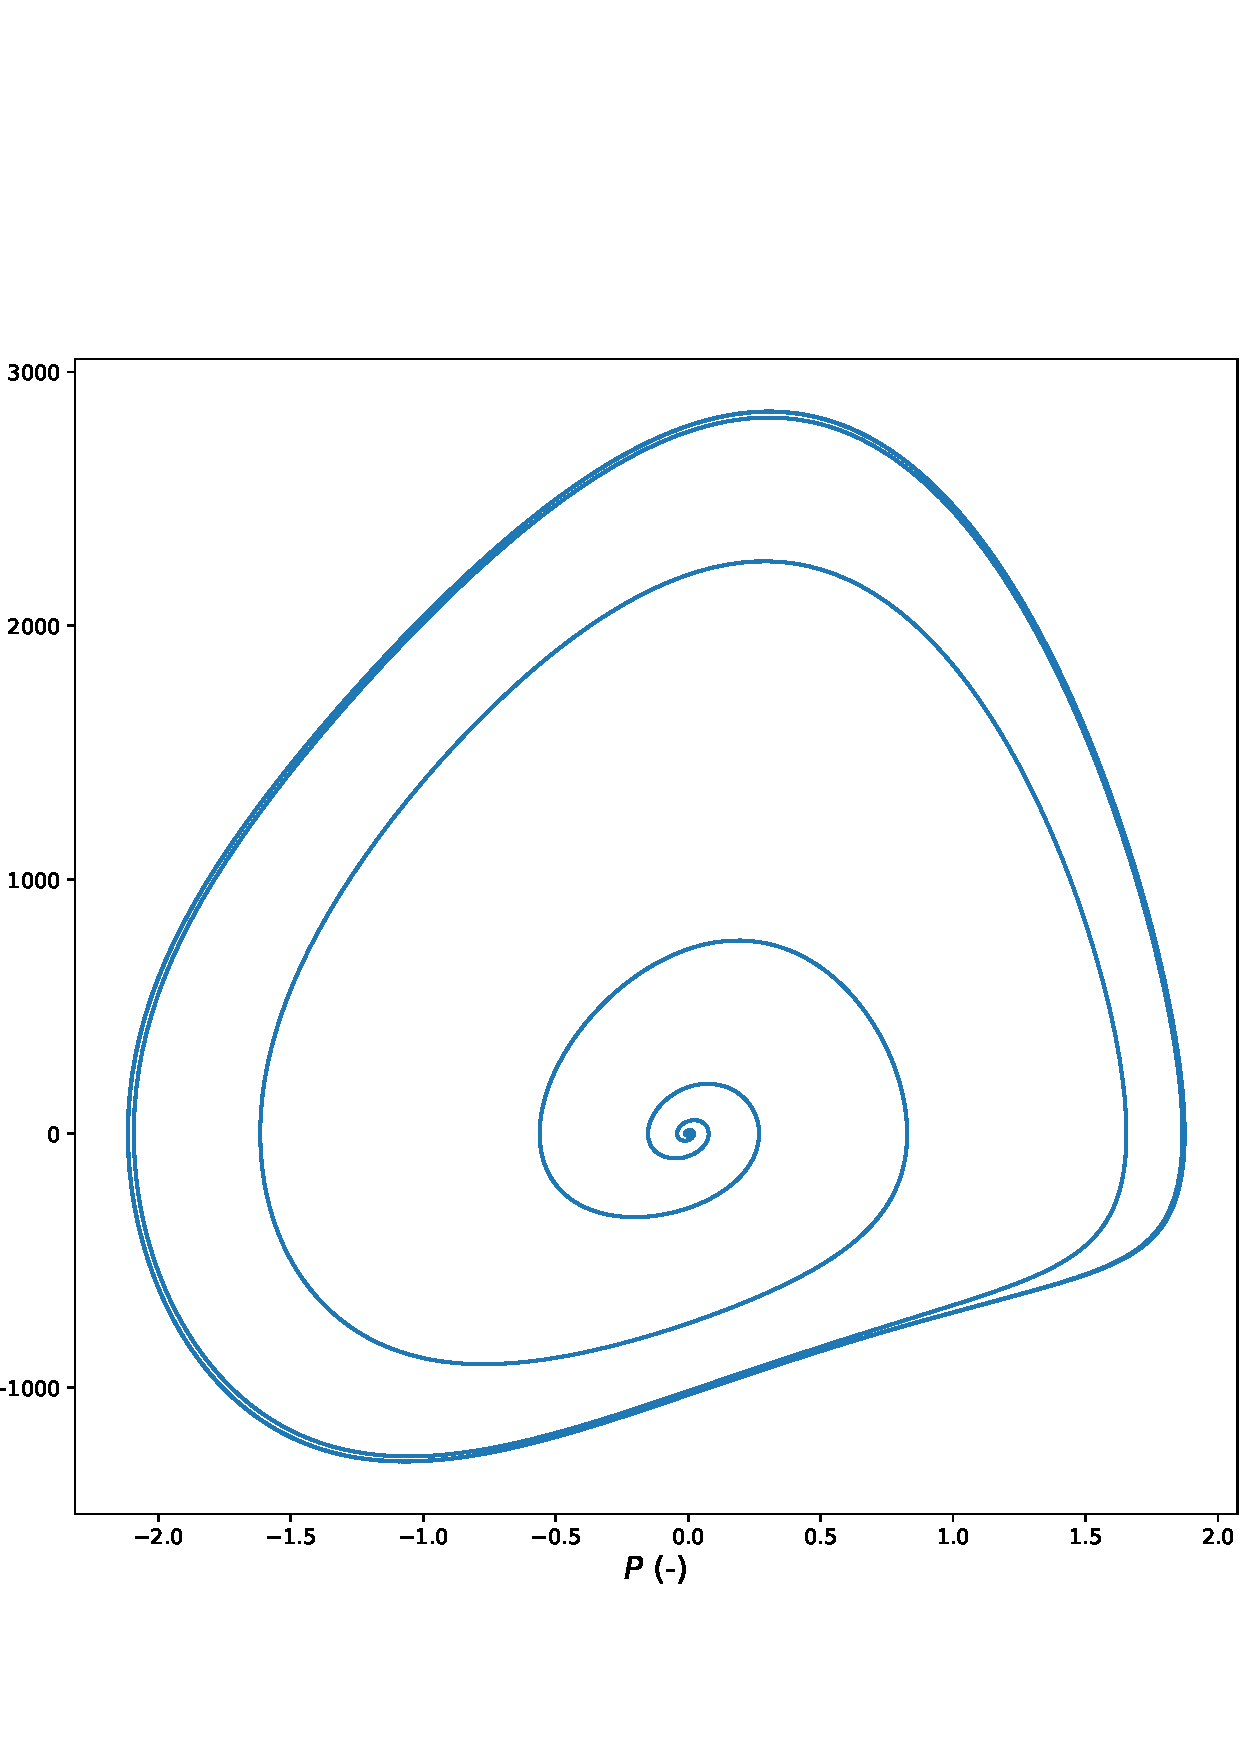
\includegraphics[width=\linewidth]{img/phase_diagram_N1.pdf}
        \caption{$N=1$}
        \label{fig:VDP_phase_N1}
    \end{subfigure}
    \hfill
    \begin{subfigure}[b]{.24\linewidth}
        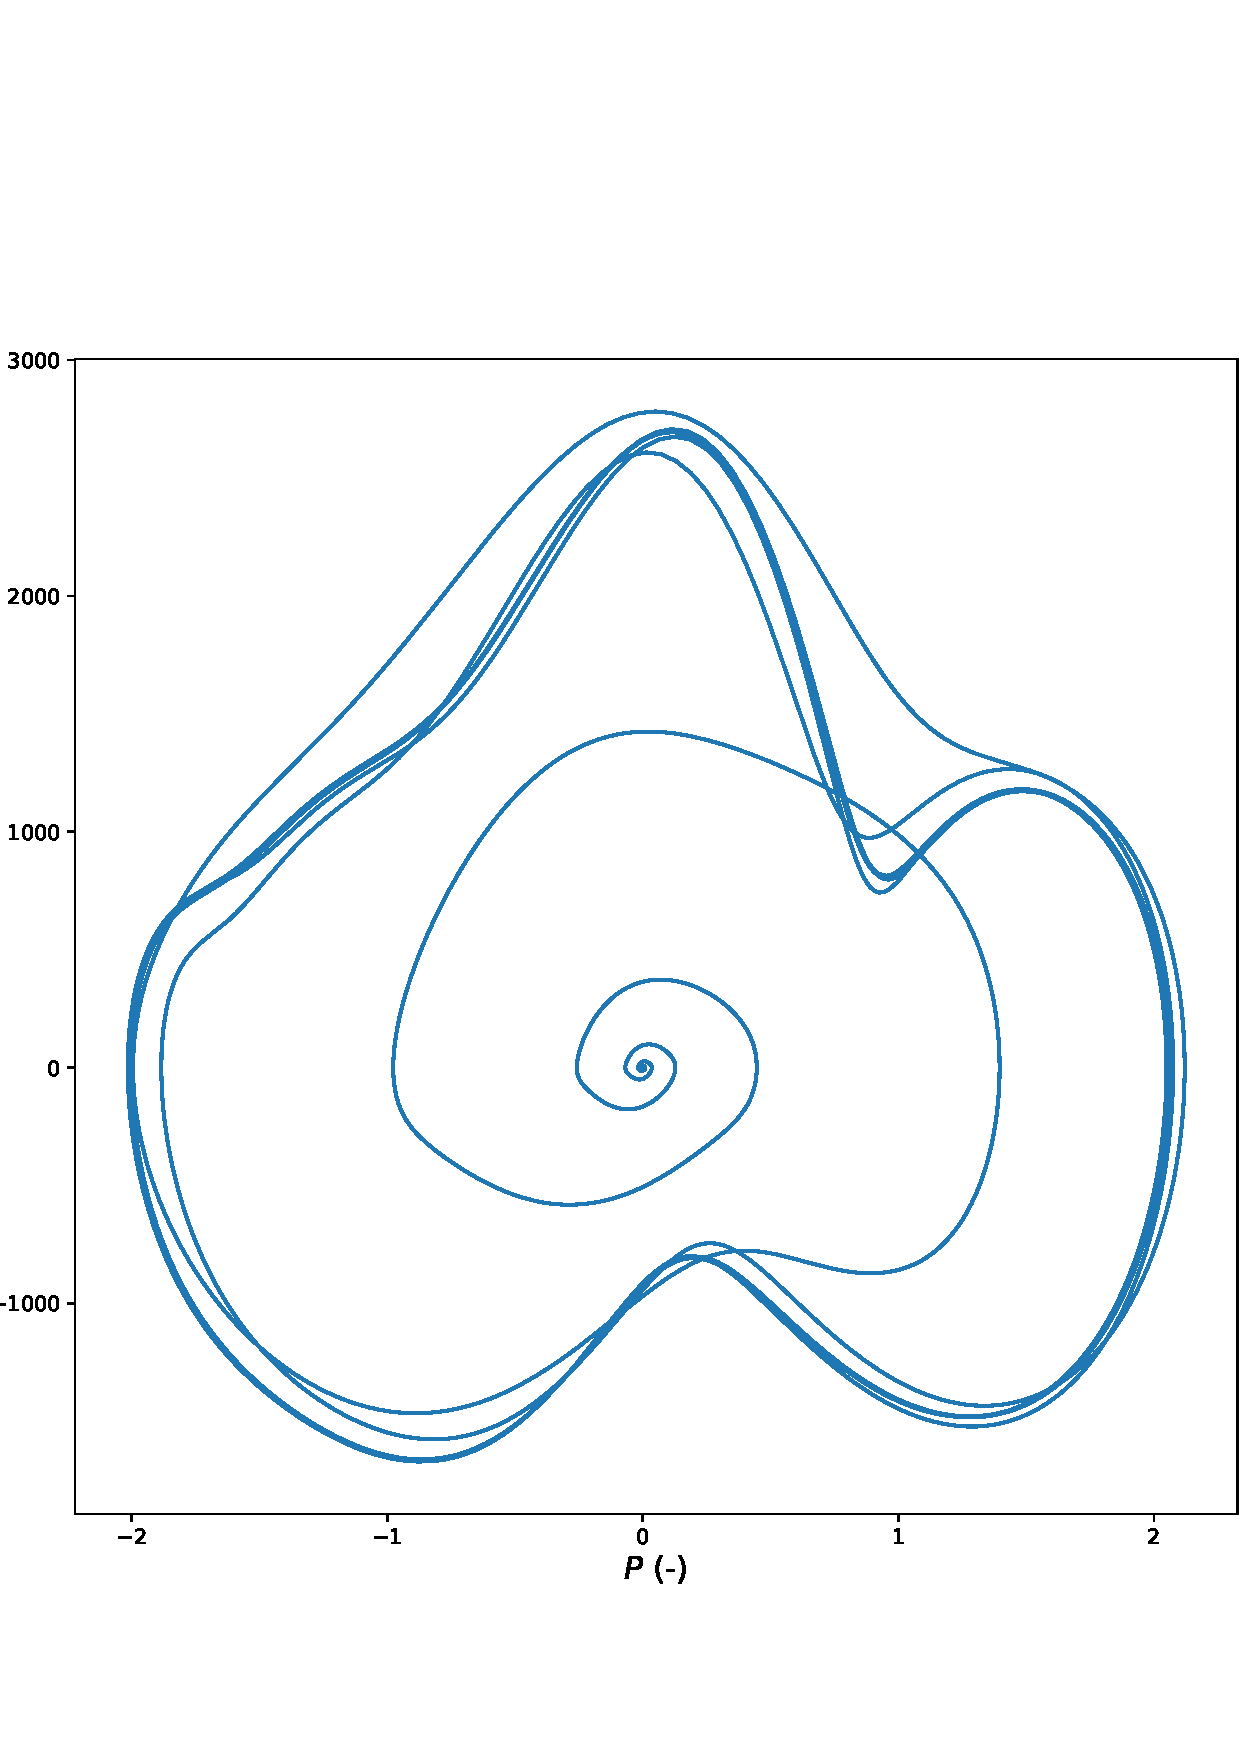
\includegraphics[width=\linewidth]{img/phase_diagram_N2.pdf}
        \caption{$N=2$}
        \label{fig:VDP_phase_N2}
    \end{subfigure}
    \hfill
    \begin{subfigure}[b]{.24\linewidth}
        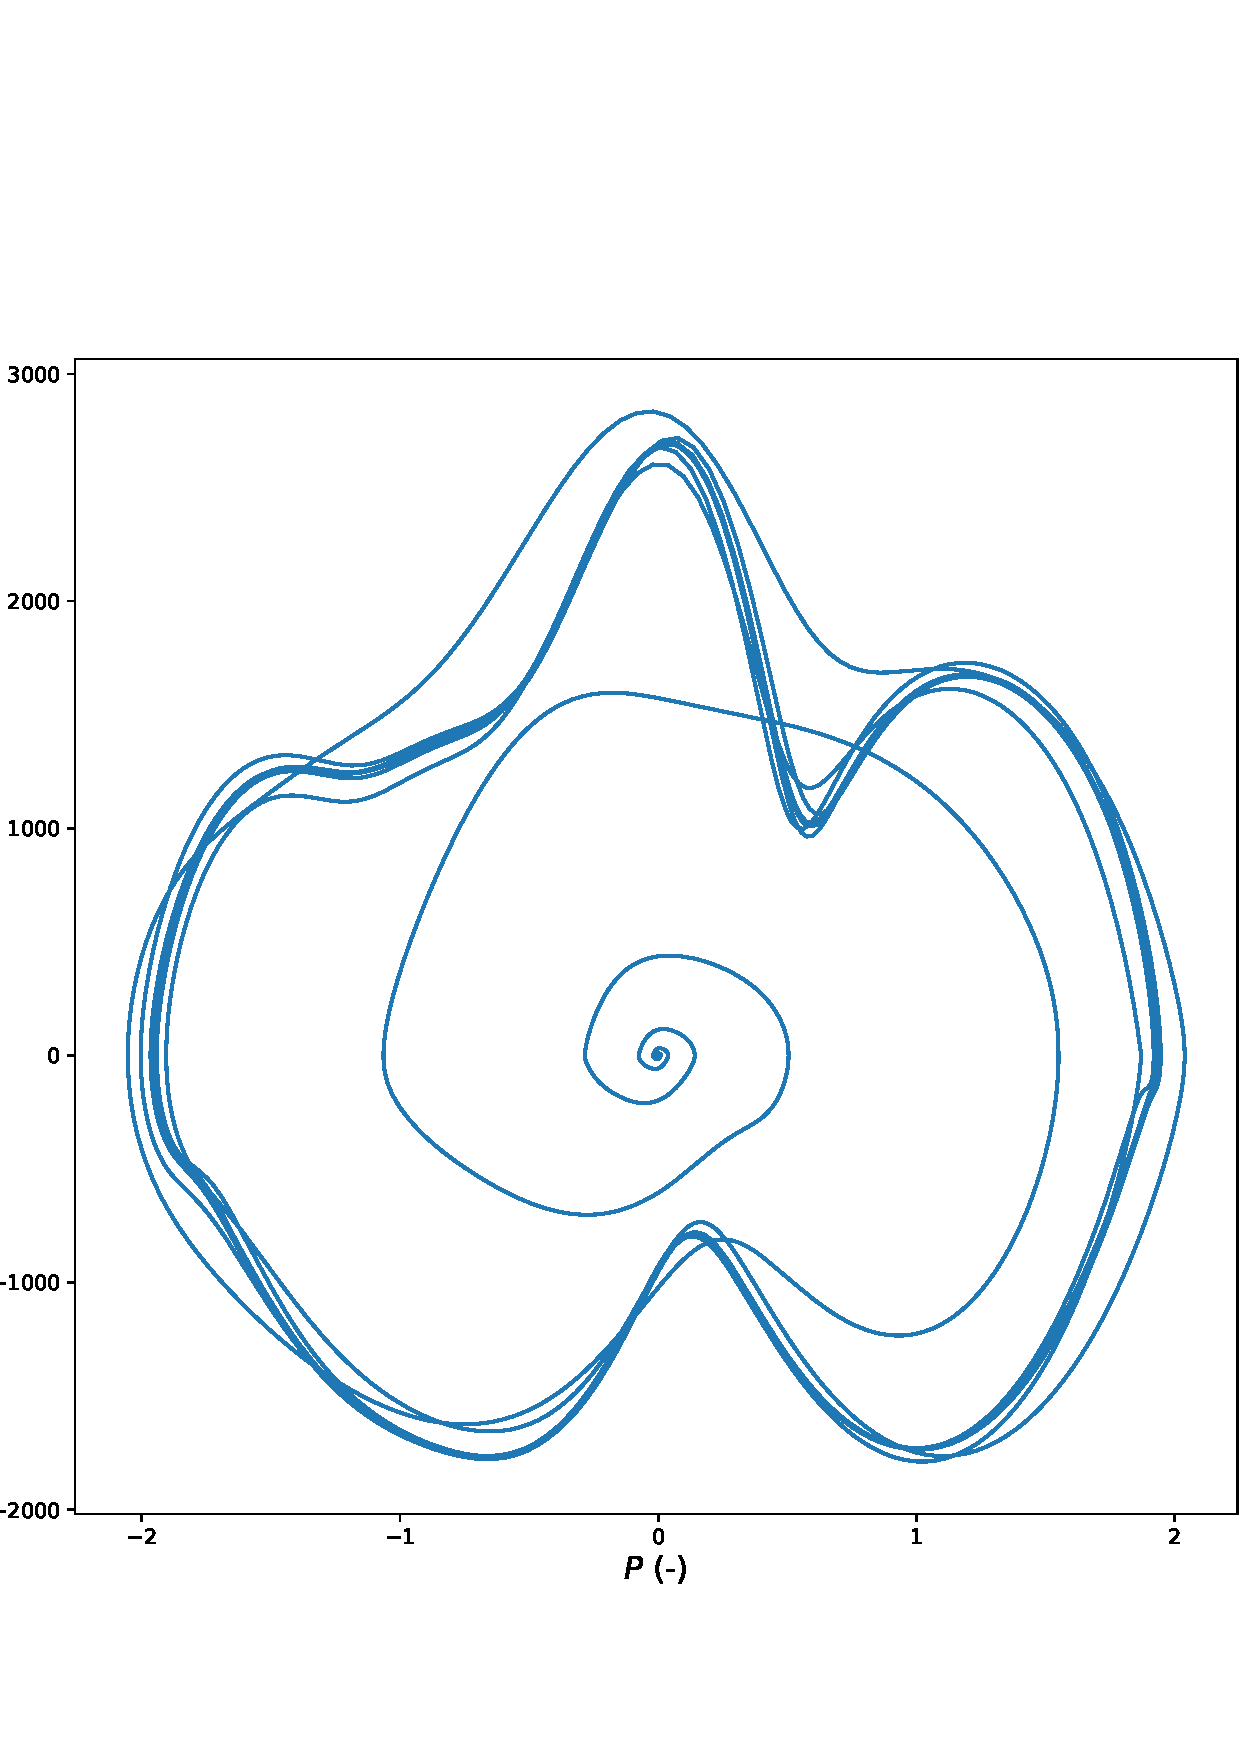
\includegraphics[width=\linewidth]{img/phase_diagram_N3.pdf}
        \caption{$N=3$}
        \label{fig:VDP_phase_N3}
    \end{subfigure}
    \hfill
    \begin{subfigure}[b]{.24\linewidth}
        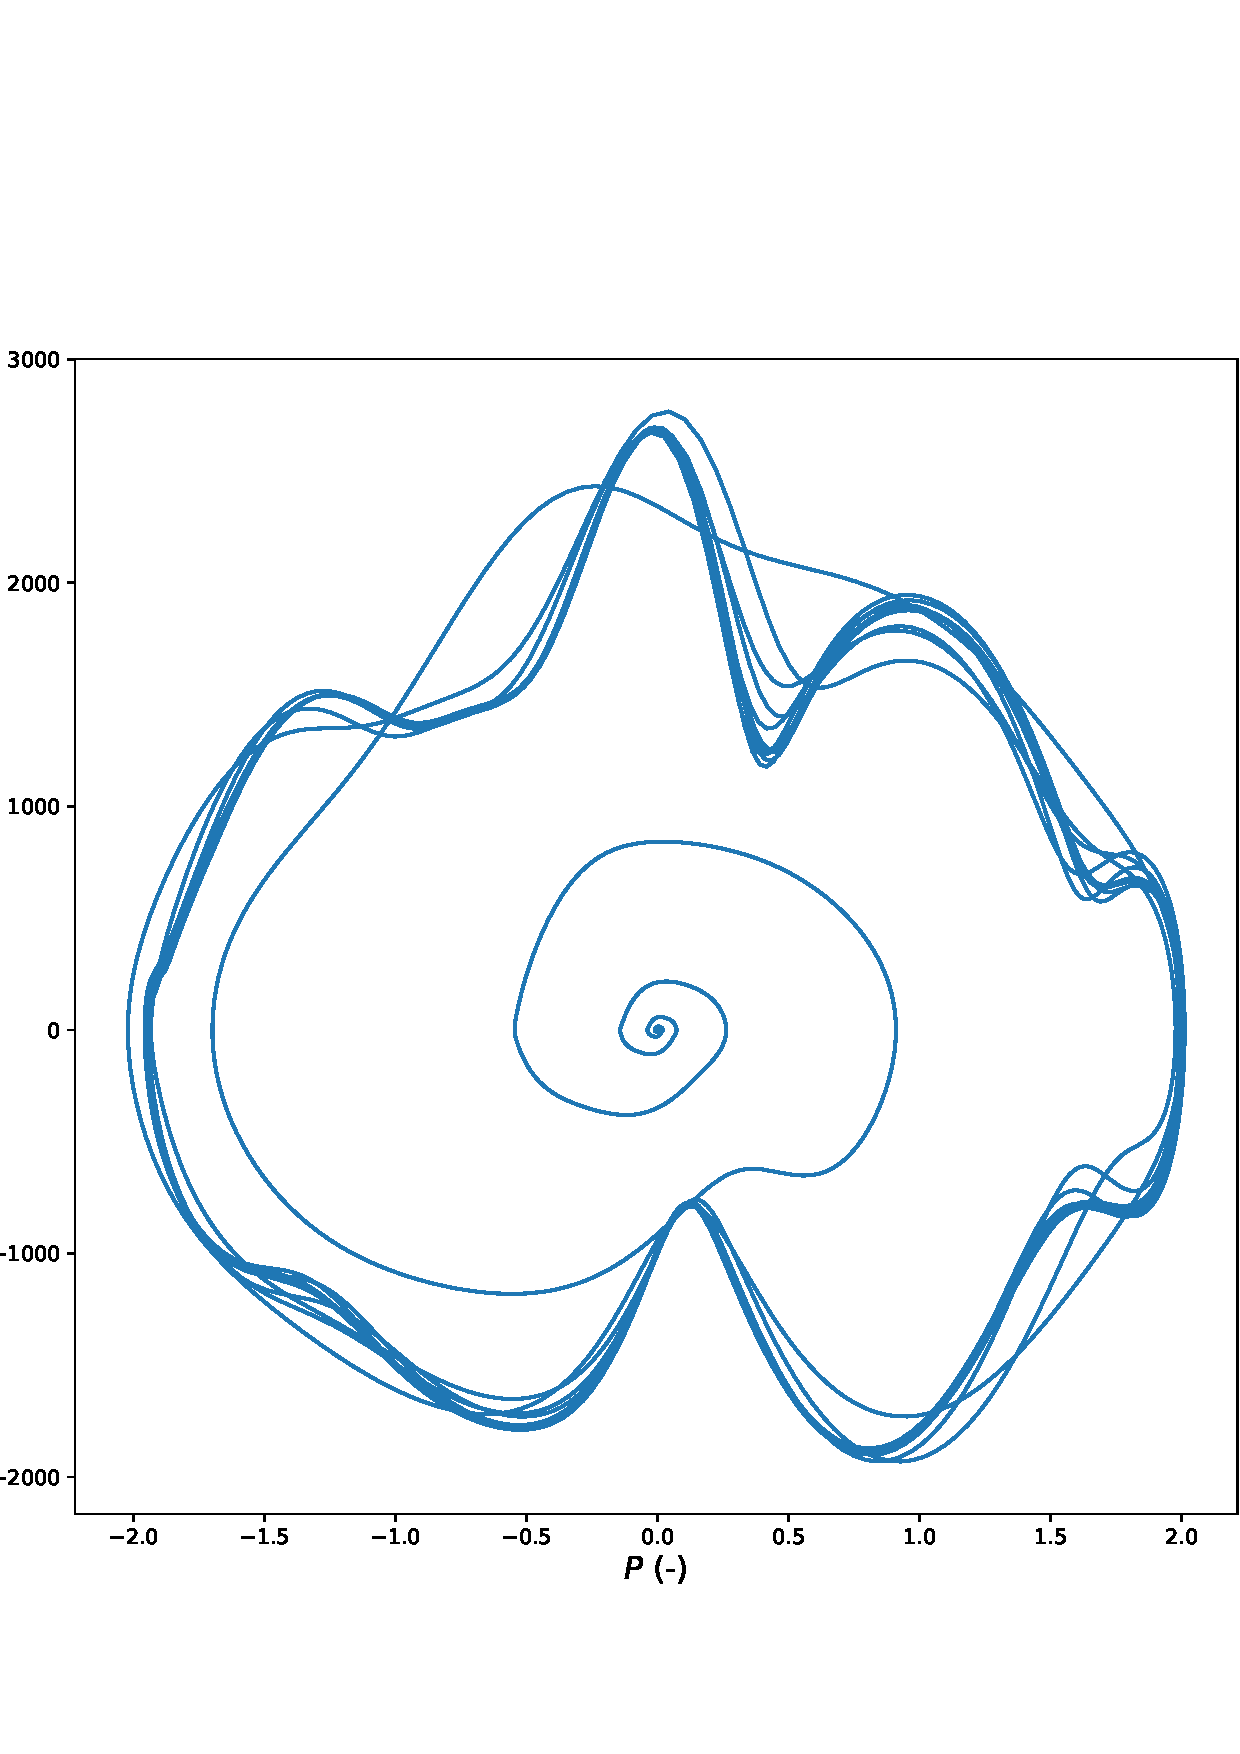
\includegraphics[width=\linewidth]{img/phase_diagram_N4.pdf}
        \caption{$N=4$}
        \label{fig:VDP_phase_N4}
    \end{subfigure}
    \caption{Evolution du flot $(P_0,\frac{\partial P_0}{\partial t})$ dans l'espace des phases durant l'attaque ($t<0.3$ s) pour $N$ modes. Le système est initialement perturbé par un saut de pression $P(t=0)=\epsilon$ ($\epsilon \ll 1$). Les solutions du système d'équations de Van der Pol convergent vers un cycle limite, dont la forme se complexifie avec N.}
    \label{fig:VDP_phase}
\end{figure*}

- résolution numérique : runge kuta

\subsubsection{Cartes itérées}

\subsubsection{Guide d'onde}

Ligne à retard, complexification du modèle pour tenir compte des pertes plus importantes en hautes fréquences.

%\section{Implémentation des modèles physiques}


% \subsection{modélisation et résolution}
% - approches analytiques : guide d'onde et modes





\section{Études des modes de jeux du modèle physique proposé}\label{sec:descripteurs}%Etude des differents modes de jeu de l'instrument numérique implémenté
Le modèle d'instruments auto-oscillant numérique présenté dans les sections précédentes, du fait de ses non-linéarités, possède des modes de jeu et de régimes sonores divers \cite{missoum_explicit_2014}\cite{doc2014minimal}. On souhaite dans cette partie étudier et classifier les différents types de jeu disponibles pour cet instrument en fonction des paramètres de contrôles de l'instrument numérique : $\zeta$ et $\gamma$. 

Nous limitons notre étude dans cette partie à l'instrument virtuel type clarinette modélisé selon l'approche modale présentée précédemment. Nous prenons en compte deux modes. 

\subsection{État de l'art}

L'étude des régimes de jeux des instruments oscillants repose sur l'établissement de descripteurs permettant de décrire certains comportements de l'instrument. Nous identifions plusieurs descripteurs présentés dans la littérature dédiée. Un premier est la présence ou l'absence de son dont une définition explicite est donnée dans \cite{missoum_explicit_2014}. Un autre descripteur est la nature du régimes d'oscillation atteint dans le cas où un son est produit, par exemple, Doc, Vergez et Missoum \cite{doc2014minimal} proposent une méthode de classification et un critère d'identification des régimes quasi-périodique pour les instruments auto-oscillants.
On peut également étudier la justesse de l'instrument numérique par rapport aux fréquences propres du résonateur \cite{missoum_explicit_2014}. 
La relation entre ces trois descripteurs et les sons produits par des instruments numériques tels que la clarinette ont fait l'objet d'articles. 
Cependant, de nombreux autres descripteurs permettant d'évaluer la sonorité d'instruments de musique existent tels que la clarté ou encore la rugosité qui est définie par rapport aux amplitudes des différentes composantes fréquentielles d'un son \cite{pressnitzer1998perception}. 
%\paragraph{Espace de phase}
Gibiat \cite{gibiat_phase_1988} propose d'utiliser la représentation en espace des phases accompagnée d'une analyse de Fourier pour détecter le comportement multiphonique d'une clarinette. Cette représentation est obtenue en traçant l'évolution des degrés de liberté du système ou dans le cas d'une réduction à un degré de liberté principal, la représentation du degré de liberté aux instants $t$ et $t + \tau$. 

Pour certains descripteurs (comme la présence de son), il est possible d'obtenir une solution analytique de la frontière entre les deux régimes. Il est également possible de prédire la nature des régimes d'oscillations de façon analytique \cite{chaigne2008acoustique}. Cependant, cette méthode permet seulement d'identifier des régimes statiques ou périodiques. Ainsi les méthodes analytiques sont limitées et ne permettent pas de décrire la diversité sonore et celle des régimes des instruments auto-oscillants. Plus récemment, l'utilisation de machines à vecteurs de support (SVM pour \textit{Support Vector Machine}) ont permis de cartographier une plus grande diversité de régimes. De plus, une méthode d'échantillonage adaptatif de l'espace des paramètres est particulièrement efficace d'un point de vue computationel et apporte des résultats beaucoup plus précis qu'un échantillonnage régulier \cite{missoum_explicit_2014}.



\subsection{Méthode}
Afin d'étudier la diversité des modes de jeu de l'instrument numérique proposé, nous présentons des descripteurs pertinents pour l'analyse des son produits par la clarinette, puis dans un second temps, nous présentons la méthode de carthographie utilisée pour étudier ces descripteurs dans l'espace $\gamma$, $\zeta$. 

\paragraph{Descripteurs utilisés}
Certains descripteurs tels que la présence de son, la périodicité et la justesse ont fait l'objet d'études ayant proposé des cartographies de ces descripteurs dans l'espace $\gamma$, $\zeta$, pour la clarinette, à partir de modèles numériques \cite{missoum_explicit_2014}, \cite{doc2014minimal}. 

La présence de son est définie comme \cite{missoum_explicit_2014}: 

\begin{equation*}
    \frac{1}{N}\sum_{N}p(t_i)>\epsilon \quad \text{Présence de son,}  
\end{equation*}
\begin{equation*}
    \frac{1}{N}\sum_{N}p(t_i)<\epsilon  \quad \text{Absence de son.}  
\end{equation*}

Le paramètre $\epsilon$ est un seuil choisi arbitrairement. L'expression théorique de la frontière entre présence et absence de son nous a permis de fixer ce seuil $\epsilon = 0.1$. 

Pour étudier la justesse, on définit l'intervalle entre deux notes en \textit{cent} comme : 
\begin{equation*}
    i = 1200 \log_2 \left( \frac{f_1}{f_2}\right).
\end{equation*}
Nous avons défini un descripteur qui caractérise si l'écart entre la fréquence jouée par le modèle est proche, selon un intervalle défini $\epsilon$ en cent, de la fréquence correspondant au premier mode propre du résonateur. Le seuil de justesse choisi est $\epsilon = 5 cents$ \cite{missoum_explicit_2014}. 

Pour étudier la périodicité du signal, nous avons utilisé un descripteur défini en fonction de l'enveloppe du signal de pression $pe$ \cite{doc2014minimal}: 
\begin{equation*}
    \epsilon = \log_{10}\left(\frac{Var(pe)}{\langle pe \rangle}\right)
\end{equation*}

Finalement, nous avons étudié la rugosité du son produit. Aucune définition n'a été donnée pour ce paramètre dans la littérature pour un cas d'application proche du notre. Nous avons choisi de définir la rugosité en fonction des fréquences et des amplitudes des composantes des sons ($f_i$, $a_i$) comme \cite{pressnitzer1998perception}: 
\begin{equation}
    \epsilon = \frac{\sum_{i,j =1}^{N}a_ia_jr_{i,j}}{\sum_{i=1}^{N}a_{i}^{2}}, 
\end{equation}
avec 
\begin{equation*} 
\begin{cases}
    r_{i,j} = (2,7183 \times \delta f_{norme} \times e^{-\delta f_{norme}})^2\\
    \delta f_{norme} = \frac{f_i-f_j}{cb_{i,j \times 0.25}}\\
    cb_{i,j} = 1.72 \times (\frac{f_i+f_j}{2})^{0.65} 
\end{cases}.
\end{equation*}

Le seuil a été fixé suite à l'estimation des valeurs que prend la rugosité sur l'espace des paramètres de contrôle dont les résultats seront présentés ci-dessous. 

\paragraph{L'espace de phase}\label{par:espace de phase}

La représentation dans l'espace des phases propose une lecture graphique intéressante des phénomènes vibratoires de la clarinette. La figure \ref{fig:phase-reg-1}, présente la représentation dans l'espace de phase d'un Ré premier registré joué à la clarinette, la figure \ref{fig:phase-reg-2}, celle d'un La deuxième registre. On observe que les deux formes sont de complexités très différentes, il semble alors intéressant d'essayer de construire un descripteur permettant d'analyser la complexité des son produits par le modèle grâce à la représentation dans l'espace de phase. 
Une première tentative à été d'essayer de construire un descripteur pour identifier le registre utilisé sur des enregistrements réels où cette information nous est connue. 
Malheureusement, même si deux registres se distinguent bien graphiquement, il a été difficile de construire un algorithme simple pour distinguer les registres les uns des autres. Deux tentatives ont été menées : la première consistait à compter le nombre de points à vitesse lente (en dessous d'un seuil), mais cette méthode était trop sensible à de faibles variations de timbre. La deuxième consistait à colorier une image avec la courbe obtenue en considérant le nombre de pixels coloriés (plus cette valeur est grande, plus la trajectoire est irrégulière). Malheureusement, cette information n'était pas suffisante pour extraire des informations fiables.

Bien qu'intéressant, nous n'avons pas étudié l'influence des paramètre de contrôle sur la représentation dans l'espace de phase des signaux. 

\begin{figure}[h!]
    \centering
    \begin{subfigure}[b]{0.9\linewidth}
        \includegraphics[width=\columnwidth]{Descripteurs/images/espace_des_phases_premier_registre.pdf}
        \caption{Note Ré (premier registre)}
        \label{fig:phase-reg-1}
    \end{subfigure}
    \hfill
    \begin{subfigure}[b]{0.9\linewidth}
        \centering
        \includegraphics[width=\columnwidth]{Descripteurs/images/espace_des_phases_second_registre.pdf}
        \caption{Note La (deuxième registre)}
        \label{fig:phase-reg-2}
    \end{subfigure}
    \caption{\emph{Portraits de phases}.}
\end{figure}

\vspace{3cm}

\paragraph{Méthode de cartographie de l'espace des paramètres en fonction des descripteurs : SVM à échantillonnage adaptatif de l'espace des paramètres.}

Bien souvent, les descripteurs sont longs à évaluer pour des raisons de temps de calcul. Ainsi, un grand nombre d'évaluations n'est pas possible pour cartographier l'espace des paramètres. Une manière d'interpoler les descripteurs sur l'espace des paramètres échantillonné grossièrement est de d'utiliser une SVM (\textit{support vector machine}). Cette dernière fait apparaître une frontière de décision continue permettant d'interpoler les descripteurs sur l'espace des paramètres. %qui est meilleure que d'utiliser la valeur du voisin le plus proche.  
On définit la frontière entre deux classes : $y = \pm1$, pour un nombre $N$ d'échantillons $\mathbf{x_i}$ comme : 
\begin{equation}
    s(\mathbf{x}) = b + \sum_{i=1}^{N}\lambda_iy_iK(\mathbf{x_i},\mathbf{x}) = 0. 
\end{equation}
On note $b$, le biais, $\lambda_i$ le multiplicateur de Lagrange. 
$K$, la fonction noyau est définie comme : 
\begin{equation*}
    K(\mathbf{x_i},\mathbf{x_j}) = \exp\left(-\frac{||\mathbf{x_i}-\mathbf{x_j}||^2}{2\sigma}\right).
\end{equation*}
Nous avons ensuite utilisé la bibliothèque \href{https://scikit-learn.org/}{scikit-learn} de python pour implémenter la SVM. 

En général, une cartographie peut être réalisée en quadrillant l'espace des paramètres et en évaluant les descripteurs en un point de chaque cellule. Cependant, pour éviter d'avoir recours à un quadrillage trop fin, une méthode d'échantillonnage adaptatif est employée \cite{missoum_explicit_2014}\cite{basudhar2008adaptive}. Cette méthode consiste à choisir un point $\mathbf{x}$ sur la frontière tel que son plus proche voisin est le plus loin. Cela revient à optimiser la minimiser l'expression suivante : 
\begin{equation*}
     \max_{\mathbf{x}} || \mathbf{x}-\mathbf{x_p}||, \quad
      \text{t. q.} ~~~s(\mathbf{x}) = 0 . 
\end{equation*}

\subsection{Résultats}
Nous avons effectué des cartographies par SVM à échantillonnage adaptatif pour les descripteurs de présence de son, de justesse et d'harmonicité \ref{fig:cartographies}. 
L'étude de la présence de son en fonction des paramètres de contrôle $\zeta$ et $\gamma$ \ref{subfig:son} montre qu'il est possible de produire du son avec l'instrument numérique à partir de $\gamma=0.33$. Plus les valeurs de $\zeta$ proches de zéro, plus la valeur seuil de $\gamma$ pour obtenir du son augmente. Ce résultat correspond à la littérature et à l'expression théorique de la frontière son/pas de son \cite{missoum_explicit_2014}. Ce premier résultat permet de confirmer à la fois la validité du modèle théorique, de notre implémentation, de la résolution numérique et du seuil choisi de $\epsilon = 0.1$ pour la cartographie. 

L'étude de la périodicité en fonction des paramètres de contrôle montre que la zone de périodicité concorde avec la zone de présence de son, sauf pour les valeurs extrêmes $\gamma \to 1$, $\zeta \to 0$ et $\gamma \to 1$, $\zeta \to 1$, c'est-à-dire des conditions de contrôles extrêmes \ref{subfig:periodicité}. Cependant, il est important de noter que nous n'avons pas retrouvé de présence de régime quasi-périodique, telles qu'identifiés dans \cite{doc2014minimal}. Cela peut être à cause d'une différence d'implémentation ou bien à une différence de seuil dans le descripteur. 

L'étude de la justesse \ref{fig:Justesse} permet d'identifier une zone dans laquelle l'instrument joue à 5 cents près de la fréquence de résonance du premier mode du résonateur de l'instrument. Ce résultat est cohérent avec la littérature \cite{missoum_explicit_2014}. On note cependant que la zone de justesse s'étant jusqu'à des valeurs de $\zeta = 0.5$ et non $\zeta = 1$. 

\begin{figure}[h!]
    \centering
    \begin{subfigure}[b]{.49\linewidth}
        \includegraphics[width=\linewidth]{img/sonV2.png}
        \caption{Présence de son, $\epsilon = 0.1$}
        \label{subfig:son}
    \end{subfigure}
    \hfill
    \begin{subfigure}[b]{.49\linewidth}
        \includegraphics[width=\linewidth]{img/justeV2.png}
        \caption{Justesse, $\epsilon = 5 \, cents$}
        \label{fig:Justesse}
    \end{subfigure}
    \hfill
    \begin{subfigure}[b]{.49\linewidth}
        \includegraphics[width=\linewidth]{img/periodicV2.png}
        \caption{Périodicité, $\epsilon = -2 $}
        \label{subfig:periodicité}
    \end{subfigure}
    \hfill
    \begin{subfigure}[b]{.49\linewidth}
        \includegraphics[width=\linewidth]{img/carto_tot_sauf_rugo.png}
        \caption{Son, périodicité, justesse}
        \label{subfig:tot1}
    \end{subfigure}
    \caption{\emph{Cartographies : présence de son, justesse et périodicité en fonction de $\gamma$ et $\zeta$ (SVM sur 25 échantillons initiaux puis ajout de 30 échantillons adaptatifs)}}
    \label{fig:cartographies}
\end{figure}

Nous avons ensuite étudié l'influence des paramètres de contrôle du modèle sur la rugosité des sons produits. Aucune étude n'aillant à notre connaissance encore étudié ce descripteur dans ce cadre, nous avons dans un premier temps établie une cartographie sommaire de la valeurs de la rugosité telle que nous l'avons définie en fonction des paramètres $\zeta$ et $\gamma$ \ref{subfig:Rugosité}. À partir de cette cartographie, nous avons identifié une valeur seuil : $\epsilon = 4.10$. Nous avons ensuite fait une cartographie par SVM adaptatif de ce paramètre de rugosité et nous avons comparé ce résultat aux cartographies de la justesse de la présence de son et de la périodicité \ref{fig:rugo_cartoto}. La zone de rugosité se situe aux niveau des valeurs porches de 1 de $\zeta$ et $\gamma$.  

\begin{figure}[h!]
    \centering
    \begin{subfigure}[b]{.49\linewidth}
        \includegraphics[width=\linewidth]{img/rugo_colormap.png}
        \caption{Évolution de la rugosité du son en fonction de $\zeta$ et $\gamma$}
        \label{subfig:Rugosité}
    \end{subfigure}
    \hfill
    \begin{subfigure}[b]{.49\linewidth}       
        \includegraphics[width=\linewidth]{img/carto_tot.png}
        \caption{Rugosité comparée aux cartographies \ref{subfig:tot1}}
        \label{fig:rugo_cartoto}
    \end{subfigure}
    
    \caption{\emph{Cartographie de la rugosité du son en fonction de $\gamma$ et $\zeta$}}
    \label{fig:cartographies}
\end{figure}

Les cartographie obtenues dans cette partie permettent de définir, en fonction des paramètres de contrôle de l'instrument, différents types de son produits. Au delà d'informer sur le fonctionnement de l'instrument numérique implémenté, elles ont vocation à servir de support l'interface en temps réelle, délimitant des zones de navigation contraintes par les frontières définies par les cartographies. 


\section{Contrôle}

\subsection{État de l'art}

Plusieurs outils de programmation d'applications musicales interactives sont disponibles et ont été utilisés avec succès pour de précédents travaux. 
Nous pourrons citer 
\href{https://cycling74.com/products/max}{Max},
\href{https://faust.grame.fr/}{Faust}
et 
\href{https://puredata.info}{Pure Data}
comme principaux choix pour réduire la complexité des implémentations et permettant de travailler uniquement sur les algorithmes de traitement et les interfaces utilisateur. 
Pour un embarquement dans un microcontroleur et gagner l'autonomie de l'instruments, plusieurs solutions existent offrant la possibilité de travailler avec les outils susnommés comme le projet \href{https://electro-smith.com/}{Daisy}.


\subsection{Implémentation et interface temps réel}

Pour cette étude a été choisi de réaliser l'application à l'aide de Max-MSP, offrant un environnement de programmation visuelle orienté vers les traitements numériques audio en temps réel et l'intéractivité avec l'utilisateur. 
Pour implémenter la méthode de Runge-Kutta \ref{sec:result_modal} à l'ordre quatre, il est nécessaire de traiter chaque échantillon du signal indépendemment.
Pour cela, Max propose l'environnement Gen qui, en plus de répondre à cette contrainte, offre une interface textuelle simplifiant l'implémentation.
Enfin, pour l'interface, l'intégration de Javascript dans le \textit{patch} étend les possibilités d'interaction avec l'utilisateur.
Il sera utilisé pour contraindre les paramètres de jeu dans les intervalles de validité de certains critères en fonction des choix de l'utilisateur.
Deux applications on été réalisées basées sur les deux modèles de synthèse abordés dans cette étude.


% @TODO Mettre éventuellement un lien vers un drive avec des sons ou des vidéos


\begin{comment}
    brouillon d'abstract
\end{comment}



% \section{Méthodes et résultats}
% \subsection{Méthode}




% \subsubsection{Méthode d'évaluation du dispositif}

%\subsubsection{cartographie}
% \section{Évaluation du dispositif}
% apprécier en situation de jeu/intérêt de l'intérêt : évaluation de l'instrument créé. (réalisme, jouabilité, compréhension de la physique : outil didactique)  
\newpage

\section{Conclusion et perspectives}

\begin{comment}
    axe d'approche "type PAM"
        aborder les éléments appris pendant le projet en plus des contributions.
\end{comment}
Durant ce projet, nous avons :
\begin{enumerate}
    \item étudié différentes modélisations d'instruments auto-oscillants ;
    \item proposé un modèle d'instruments numérique ;
    \item contrôlé en temps réel sous Max/MSP ;
    \item étudié les différents régimes de jeu de cet instrument numérique.
\end{enumerate}


Nous nous sommes intéressés dans ce projet aux modèles d'instruments auto-oscillants à anche simple type clarinette ou saxophone. Nous avons modélisé ces instruments selon deux approches : par méthode de guide d'ondes et par approche modale. Nous avons proposé une implémentation en temps réel de ces deux approches. 

L'approche par guide d'ondes nous a permis d'identifier des régimes tels que le doublement de périodes et le quadruplement de périodes. Un inconvénient de ce modèle est la forme d'onde rectangulaire de ses solutions, produisant un son synthétisé qualitativement peu réaliste.  D'un autre côté, l'approche modale donne un rendu sonore qualitativement plus réaliste que l'approche par guides d'onde.
%Mentionner : - approche modale -> timbre pas mal
%- approche carte itérée : apparition de davantage de régimes intéresse


Nous avons également proposé d'étudier l'influence des paramètres de contrôle $\zeta$ et $\gamma$ sur la production de son, la justesse, la rugosité et la périodicité des son produits par l'instrument numérique, basé sur le modèle physique par approche modale. Si notre travail a permis de retrouver les résultats de la littérature quant aux conditions de production de son du modèle, il nous a également permis de proposer une cartographie de la rugosité en fonction des paramètres de contrôle. 


Nous avons ensuite utilisé ces cartographies pour informer l'utilisation de l'implémentation en temps réelle du modèle. Ainsi, l'utilisateur de l'instrument numérique via l'interface sous Max/MSP peut naviguer dans l'espace des paramètres de contrôle par rapport aux informations proposées via les cartographies. 

L'implémentation sur Max/MSP des deux algorithmes de synthèse résulte en deux applications intuitives à utiliser avec deux interfaces identiques. L'utilisateur peut contrôler les paramètres de jeux à l'aide d'une tablette graphique et d'un clavier MIDI et générer des sons similaires à ceux générés par les méthodes en temps différé.

La perspective principale de ce projet serait d'élargir notre travail à d'autres instruments auto-oscillants tels que le violon ou le saxophone, à la fois en étudiant les différents régimes de jeux de ces instruments et en proposant des implémentions en temps réel de ces derniers. L'utilisation de modèles d'instruments plus complexes, notamment par la prise en compte de la dynamique de l'anche, est également envisageable. Il serait également intéressant de proposer aux utilisateurs un contrôle plus direct des caractéristiques sonores produites. 
%Perspectives : rappel de l'état de l'art pour adapter notre travail à un instrument à cordes frottées -> perspective logique pour appliquer le travail à d'autres instruments (à voir si on peut utiliser l'approche modale ou si l'analogie est vraie qu'en guide d'ondes).

%- contrôle plus direct des descripteurs (volume à fréquence constante par exemple), mais nécessite une autre approche que celle utilisée ici. 


\fancypagestyle{plain}{plain}
 {\hypersetup{hidelinks} \printbibliography }


\end{document}